\documentclass[border=10pt]{standalone}
\usepackage[svgnames]{xcolor}
\usepackage{amsmath}
\usepackage{pgfplots}
\pgfplotsset{compat=newest}
\usepackage[sfdefault]{FiraSans}
\usepackage{FiraMono}
\renewcommand*\familydefault{\sfdefault}
\begin{document}
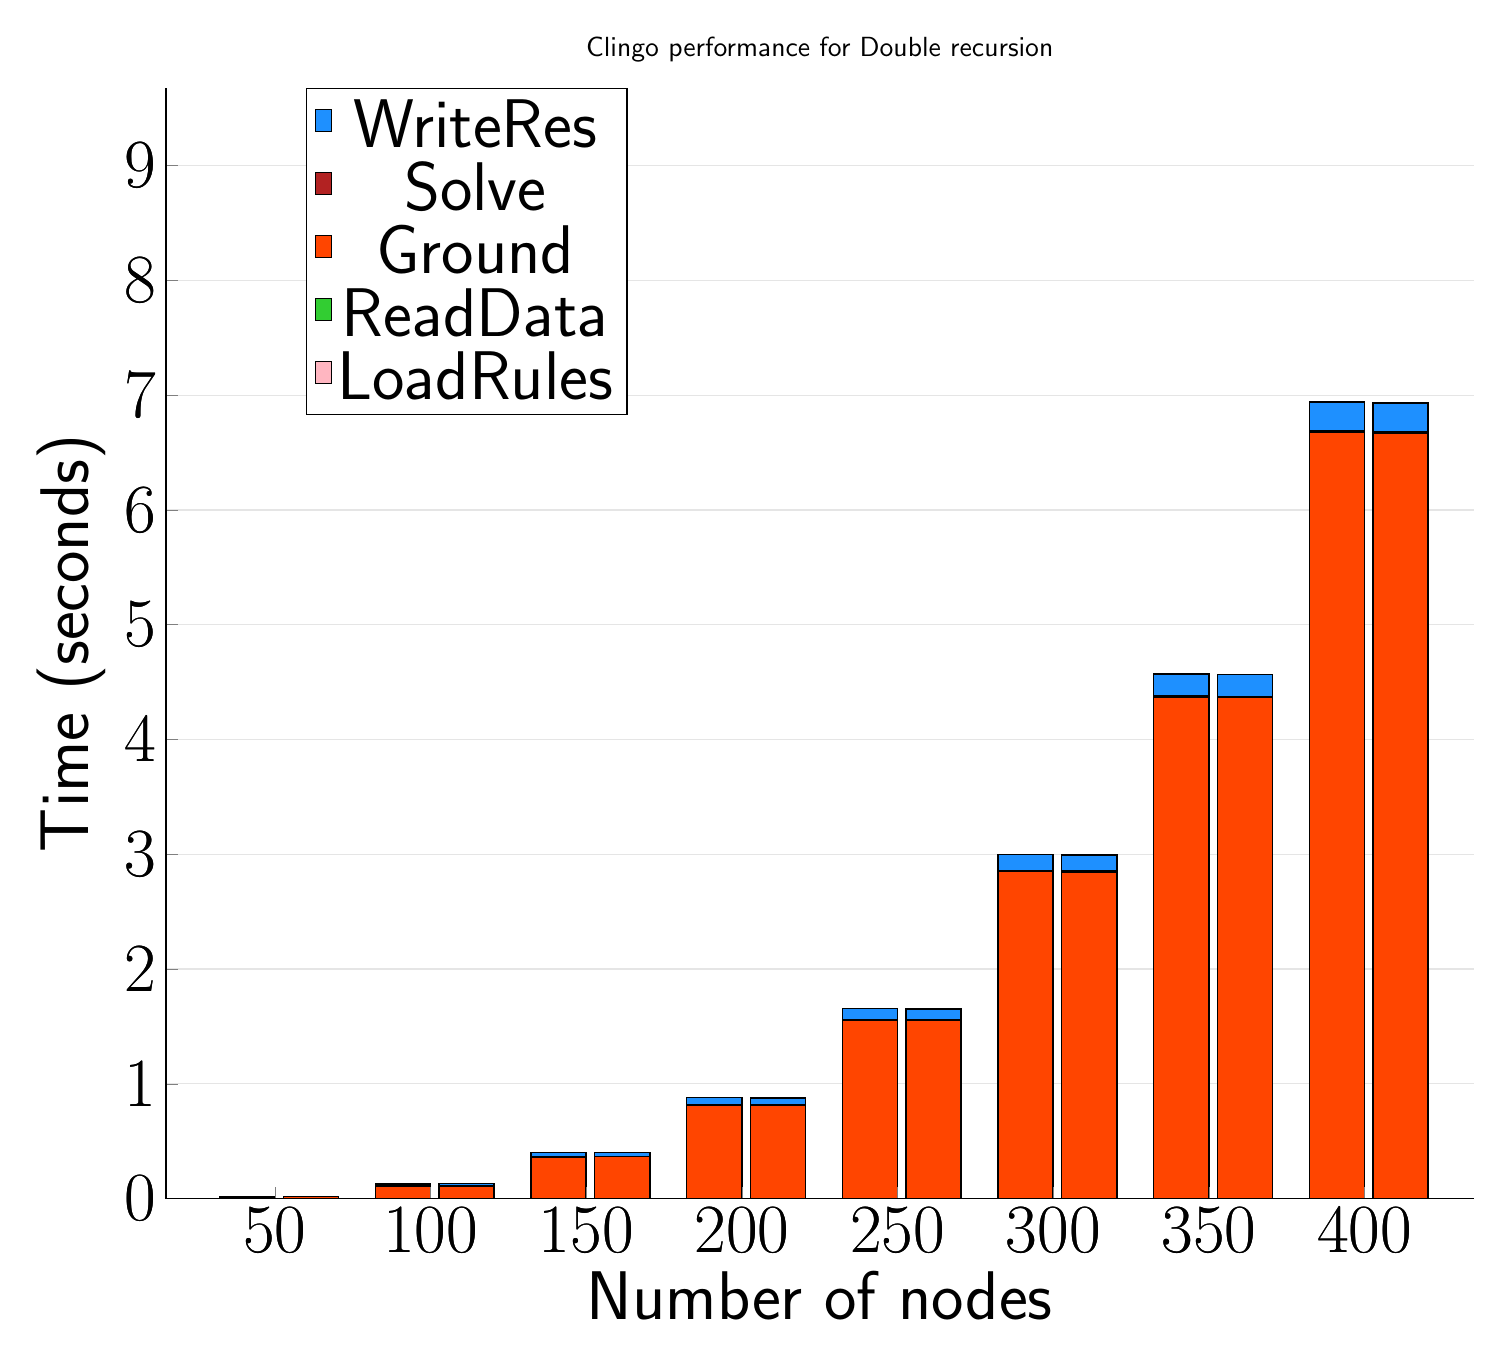
\begin{tikzpicture}
\begin{axis}[
   ybar stacked,
   title={Clingo performance for Double recursion},
   bar shift=-10pt,
   width=1.5\textwidth,
   bar width=0.7cm,
   ymajorgrids, tick align=inside,
   major grid style={draw=gray!20},
   xtick=data,
   ymin=0, ymax=9.677999997138977,
   axis x line*=bottom,
   axis y line*=left,
   enlarge x limits=0.1,
   legend style={
       at={(0.23, 1)},
       anchor=north,
       legend columns=1,
       font=\Huge,
   },
   ylabel={Time (seconds)},
   xlabel={Number of nodes},
   label style={font=\Huge},
   tick label style={font=\Huge},
]
\addlegendimage{fill=DodgerBlue, draw=black, line width=0.2pt}
\addlegendentry{WriteRes}
\addlegendimage{fill=FireBrick, draw=black, line width=0.2pt}
\addlegendentry{Solve}
\addlegendimage{fill=OrangeRed, draw=black, line width=0.2pt}
\addlegendentry{Ground}
\addlegendimage{fill=LimeGreen, draw=black, line width=0.2pt}
\addlegendentry{ReadData}
\addlegendimage{fill=LightPink, draw=black, line width=0.2pt}
\addlegendentry{LoadRules}
\addplot +[fill=LightPink, draw=black, line width=0.5pt] coordinates {
    (50, 0.0)
    (100, 0.0)
    (150, 0.0)
    (200, 0.0)
    (250, 0.0009999990463256836)
    (300, 0.0)
    (350, 0.0)
    (400, 0.0)
};
\addplot +[fill=LimeGreen, draw=black, line width=0.5pt] coordinates {
    (50, 0.0)
    (100, 0.0009999990463256836)
    (150, 0.0)
    (200, 0.0)
    (250, 0.0)
    (300, 0.0009999990463256836)
    (350, 0.0009999990463256836)
    (400, 0.0)
};
\addplot +[fill=OrangeRed, draw=black, line width=0.5pt] coordinates {
    (50, 0.014999985694885254)
    (100, 0.10900003910064697)
    (150, 0.3629999876022339)
    (200, 0.8149999856948853)
    (250, 1.5539999961853028)
    (300, 2.8509999990463255)
    (350, 4.365999984741211)
    (400, 6.677999997138977)
};
\addplot +[fill=FireBrick, draw=black, line width=0.5pt] coordinates {
    (50, 0.0)
    (100, 0.0009999990463256836)
    (150, 0.0019999980926513673)
    (200, 0.0029999971389770507)
    (250, 0.004999995231628418)
    (300, 0.008999991416931152)
    (350, 0.011999988555908203)
    (400, 0.01399998664855957)
};
\addplot +[fill=DodgerBlue, draw=black, line width=0.5pt] coordinates {
    (50, 0.005000019073486328)
    (100, 0.015999984741210938)
    (150, 0.035000038146972653)
    (200, 0.06400001049041748)
    (250, 0.09600002765655517)
    (300, 0.13599998950958253)
    (350, 0.19100000858306884)
    (400, 0.25)
};
\end{axis}
\begin{axis}[
   ybar stacked,
   bar shift=13pt,
   width=1.5\textwidth,
   bar width=0.7cm,
   ymajorgrids, tick align=inside,
   major grid style={draw=none},
   xtick=data,
   ymin=0, ymax=9.677999997138977,
   axis x line*=none,
   axis y line*=none,
   enlarge x limits=0.1,
   label style={font=\Huge},
   tick label style={font=\Huge},
]
\addplot +[fill=LightPink, draw=black, line width=0.5pt] coordinates {
    (50, 0.0)
    (100, 0.0)
    (150, 0.0)
    (200, 0.0)
    (250, 0.0)
    (300, 0.0)
    (350, 0.0)
    (400, 0.0)
};
\addplot +[fill=LimeGreen, draw=black, line width=0.5pt] coordinates {
    (50, 0.0)
    (100, 0.0)
    (150, 0.0)
    (200, 0.0)
    (250, 0.0)
    (300, 0.0)
    (350, 0.0)
    (400, 0.0)
};
\addplot +[fill=OrangeRed, draw=black, line width=0.5pt] coordinates {
    (50, 0.019999999999999997)
    (100, 0.11000000000000001)
    (150, 0.36399999999999993)
    (200, 0.8109999999999997)
    (250, 1.5500000000000003)
    (300, 2.8449999999999998)
    (350, 4.3660000000000005)
    (400, 6.67)
};
\addplot +[fill=FireBrick, draw=black, line width=0.5pt] coordinates {
    (50, 0.0)
    (100, 0.0)
    (150, 0.0010000000000000009)
    (200, 0.0050000000000000044)
    (250, 0.006999999999999984)
    (300, 0.010000000000000009)
    (350, 0.011000000000000055)
    (400, 0.015000000000000036)
};
\addplot +[fill=DodgerBlue, draw=black, line width=0.5pt] coordinates {
    (50, 0.0)
    (100, 0.01999999999999999)
    (150, 0.03599999999999998)
    (200, 0.05900000000000005)
    (250, 0.09399999999999997)
    (300, 0.14)
    (350, 0.18900000000000003)
    (400, 0.24600000000000008)
};
\end{axis}
\end{tikzpicture}

\end{document}
